\documentclass[10pt,a4paper]{article} %a3paper, a2paper osv.
\usepackage[utf8x]{inputenc}
\usepackage{ucs}
%Math pakker og indstillinger:
\usepackage{amsmath} %Math ting
\usepackage{amsfonts} %Math fonts og symboler
\usepackage{amssymb} %Math ting
\usepackage{amsthm}
\usepackage{boxproof}
\usepackage{pgfgantt}

%Kode i artikel:
%\usepackage{listings}
%\lstset{language=??? keyword=???}
%\lstinputlisting[language=ditSprog]{source_filename.py} %Komando til at inkludere fra fil

%Header og footer indstillinger:
\pagenumbering{arabic} %roman, Roman, alph, Alph
%\usepackage{lastpage}
%\pagestyle {headings} %Laver headings til hver side undtagen forside. defeault: afsnit navn+nr
%\usepackage{fancyhdr} %Pakke til at lave custom header og footer
%\pagestyle{fancy} %Custom header og footer
%\fancyhead[R, L] {Peter Alexander Garnæs \hfill Title} %Konstruerer header
%\fancyfoot{} %Ryder footer så vi selv kan placere pagenumber
%\fancyfoot[R] {side \thepage af \pageref{LastPage}} %Laver footer

%Side layout:
%\usepackage{fullpage} %Større marginer.
%\usepackage[top=2cm, bottom=3cm, left=3cm, right=3cm]{geometry} %individuelle marginer
%\usepackage[margin=1in, paperwidth=5.5in, paperheight=8.5in]{geometry} %Side dimensioner.

%Random ting:
\usepackage{array} %Array pakke
% \renewcommand\thesubsection{(\alph{subsection})} %Numererer subsections med bogtaver

%Grafik (billeder og figurer):
\usepackage{graphicx} %Til at indsætte billeder.
\usepackage{float} %Til at lave figures
\usepackage{pgf} %Figur pakke
\usepackage{tikz} %Tegne figur pakke
%Grafik indstillinger:
%\floatstyle{boxed} %Streg rundt om figurer
\usetikzlibrary{arrows,automata} %Til at lave state machines

%Oversættelser:
\renewcommand{\figurename}{Figur}
\renewcommand{\tablename}{Tabel}

\begin{document}
\title{\textbf{Synopsis}}
\author{Mehdi Asser Husum Nadif}
\date{\today}
\maketitle

\null
\vfill
\begin{center}
DIKU
\end{center}
\clearpage %Fjern eventuelt dette afsnit hvis du ikke ønsker fin forside
\section*{Title}
Effort to make a quick and precise clustering algorithm for 16S rRNA sequences.
\section*{Problem statement}
I will attempt to create a clustering algorithm, that can compete with, or even surpass, uClust in terms of speed, without losing precision, when working with a dataset of 500.000 RNA/DNA sequences of length 500-1500 characters.

\section*{Limitations}
\begin{enumerate}
\item I will only attempt to make a clustering algorithm that works for RNA/DNA sequences. 
\item I will assume that all biological data is correct, and will not account for any discrepancies in the given data.
\item The efficiency of my solution will be measured against the 64 bit version of uClust; Newer, more efficient algorithms will not be taken into account.
\end{enumerate}

\section*{Reason}

The amount of biological sequence data is increasing at a higher speed than the growth of computer efficiency, as predicted by Moore's Law. Algorithms that run quicker are therefore indispensable. For instance, in the Microbiology Department of the University of Copenhagen, more than 500 million unprocessed RNA and DNA sequence strings have amassed. They need to be clustered. The most efficient algorithm for clustering huge amounts of sequences is uClust \cite{Wei et al}, but it is unfortunately quite costly. 
There is therefore a need for an open source clustering algorithm that is as efficient speed- and precision wise as uClust. 

\section*{Work Plan}

I have set the following assignments for myself:
\begin{enumerate}
\item \textbf{Implement Prototype}\\
\textbf{Product:} A working clustering algorithm using the method i hope to finish with. It does not have to be quick or precise, nor parallelized, but it should be working.\\
\textbf{Resources:} C (programming language), Notepad++ as editor.\\
\textbf{Dependencies:} Analysis of clustering algorithms.\\
\textbf{Workload:} 5-7 days.
\item \textbf{Improve implementation}\\
\textbf{Product}: Improving upon the working algorithm by testing, debugging and parallellization. Might also need to improve small parts of the algorithm, such as database search and the distance metric.\\
\textbf{Resources:} C, Notepad++, Articles on optimization of database search etc.\\
\textbf{Dependencies:} A finished prototype.\\
\textbf{Workload:} 8-10 days.
\item \textbf{Write midway report}\\ 
\textbf{Product:} Having written the midway report. It should include an introduction to the subjects i've used for the prototype, such as statistics, clustering algorithms, and whatever else might be used.\\
\textbf{Resources:} Articles about the subjects that i use, Latex.\\
\textbf{Dependencies:} Analysis of clustering algorithms.\\
\textbf{Workload:} 10-15 days.\\
\item \textbf{Analysis of clustering algorithms.}\\
\textbf{Product:} An analysis of a diverse number of clustering algorithms to find out which method to use for the prototype.\\
\textbf{Resources:} Many articles about clustering.\\
\textbf{Workload:} 2 days
\item \textbf{Write rest of report}\\
\textbf{Product:} Any additional background material will be added, otherwise the analysis of the algorithms speed comparatively with other similar algorithms will be added, and the conclusion. Goes along with the improvement of the algorithm.\\
\textbf{Dependencies:} Midway Report, Prototype.\\
\textbf{Resources:} Latex, Results from tests.\\
\textbf{Workload:} 8-10 days.\\
\end{enumerate}

\begin{figure}[H]
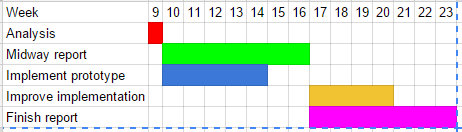
\includegraphics[scale=1]{Gantt}
\end{figure}


\clearpage
\begin{thebibliography}{9}
\bibitem{Kazimianec}
   Michail Kazimianec, Arturas Mazeika, \emph{Clustering of Short Strings in Large Databases}, 2009
\bibitem{Statistical Learning}
   Trevor Hastie, Robert Tibshirani, Jerome Friedman, \emph{The Elements of Statistical Learning: Datamining, Inference, and Prediction}, 2. ed., Springer Series in Statistics, 2008
\bibitem{clustData}
   Anil K. Jain, Richard C. Dubes, \emph{Algorithms for Clustering Data}, Michigan State University, 1988.
\bibitem{Modelbasedclust}
   Yaqing Si, Peng Liu, \emph{et al.}, \emph{Model-based clustering for RNA-seq data.}, November 4. 2013.
\bibitem{grammarbased}
   David J Russell, Samuel F Way, Andrew K Benson, Khalid Sayood, \emph{A grammar-based distance metric enables fast and accurate clustering of large sets of 16S sequences}, BMC 2010.
\bibitem{Edgar1}
   Robert C. Edgar, \emph{Search and clustering order of magnitude faster than BLAST}, 2010.
\bibitem{cdhit}
   Limin Fu, Beifang Niu, Zhengwei Zhu, Sitao Wu, Weizhong Li, \emph{CD-HIT: accelerated for clustering the next-generation sequencing data}, 2012
\bibitem{ultrafast}
  Weizhong Li \emph{et al.}, \emph{Ultrafast clustering algorithm for metagenomic sequence analysis}, 2012
\bibitem{Xiao}
  Xiao Yang, J. Zola, \emph{et al.}, \emph{Large Scale Metagenomic Sequence Clustering via Sketching and Maximal Quasi-clique Enumeration on Map-Reduce Clusters}, 2012
\bibitem{minwiseclust}
  Zeehasham Rasheed, Huzefa Rangwala, \emph{A Map-Reduce Framework for Clustering Metagenomes}, 2013
\bibitem{farrar}
  Michael Farrar, \emph{Striped Smith-Waterman speeds database searches six times over other SIMD implementations}, 2006
\bibitem{minwiseart}
  Andrei Z. Broder, \emph{et al.}, \emph{Min-Wise Independent Permutations}, 1998
\bibitem{dnaclust}
  Mohammadreza Ghodsi, Bo Liu, Mihai Pop, \emph{DNACLUST: accurate and efficient clustering of phylogenetic marker genes}, 2011
\bibitem{comparison}
  Chen W, Zhang CK, Cheng Y, Zhang S., Zhao H, \emph{A Comparison of Methods for Clustering 16S rRNA Sequences into OTUs}, 2013
\bibitem{Wei et al}
  Leonard M. Adleman, \emph{Computing with DNA}, Scientific America, 1998.
\bibitem{minmaxhash}
  Jianqiu Ji and Jianmin Li and Shuicheng Yan and Qi Tian and Bo Zhang, \emph{Min-Max Hash for Jaccard Similarity}, 2013
\end{thebibliography}
\end{document}